\section{Evaluation} \label{evaluation} 
To evaluate our continuous training approach, we perform several experiments.
We first describe the setup of our experiments including the computing cluster, the deployed pipeline, and how we simulate a real production environment by streaming a real-world large dataset through our deployment platform.
First, we discuss the effect of different parameters (learning rate adaptation, sampling strategy, and scheduling policy) on the quality and training time of the model.
Then, we discuss the effects of proactive training on the quality and freshness of the model and compare them to a model that is trained periodically.
Finally, we evaluate the training time of the continuous training approach and the effects of online statistics computation and data materialization optimizations on the training time.

\subsection{Setup}\label{subsec:setup}
We evaluate our deployment method in distributed environment consists of 21 nodes (1 master, 20 slaves).
Each node is running on an Intel Xeon 2.40 GHz 16 core processor and has 28 GB of dedicated memory for running our prototype.
We use Apache Spark 2.2.0 running on Hadoop 2.7.
We use 16 task slots per executor node (a total of 320 slots).

To demonstrate the deployment platform designed the following machine learning pipeline.

\textbf{Criteo Pipeline.} 
The Criteo pipeline consists of 5 operations: input parser, missing value imputer, standard scaler, one hot encoder, and logistic regression model trainer. 
The Terabyte Criteo click log dataset is used for benchmarking algorithms for clickthrough rate (CTR) prediction \cite{criteo-log}.
It contains 24 days of user click logs. 
The dataset contains 13 numerical and 26 categorical features. 
In all of our experiments, we are using the data from the first 3 days (Day 0 to Day 2) of the Criteo dataset.
Day 0 is used for the initial offline training of the pipeline.
The data from Day 1 and Day 2 are used as streaming data sources.
To evaluate the quality of the pipeline, we use a sample of the Day 6 to compute the logistic loss.

\textbf{Criteo Data Simulation.}
We simulate a production environment by streaming 2 days of the Criteo dataset.
The data from each day is divided into 1440 smaller batches and stored on disk.
Each batch represents one minute of data.
We use spark streaming to read the data files one by one and stream them through the deployment platform. 
All the experiments are using day 1 and day 2 as streaming sources unless specified otherwise.

\subsection{Learning Rate Adaptation Method}
In Section \ref{sgd}, we discussed the importance of learning rate tuning for training a model using the Stochastic Gradient Descent optimization method.
Proactive training is an extension of SGD, therefore the process of tuning the learning rate adaptation method is no different from tuning it for an offline SGD training.

To find the best learning rate adaptation algorithm, we first train a model using SGD optimization algorithm for 500 iterations using Adadelta, RMSprop, and Adam, three of the state of the art learning rate adaptation techniques.
After the training, the models (and the pipelines) trained with different learning rate adaptation techniques are deployed.
We use the first day of the Criteo data to investigate the effect of the learning rate adaptation techniques on Criteo pipeline.
Figure \ref{fig:criteo-learning-rate} shows the logistic loss error rate of different learning adaptation techniques. 
During the SGD training phase, we capture the logistic loss on the evaluation dataset after 20, 40, 80, 160, 320, and 500 iterations of training.


\begin{figure}[h!]
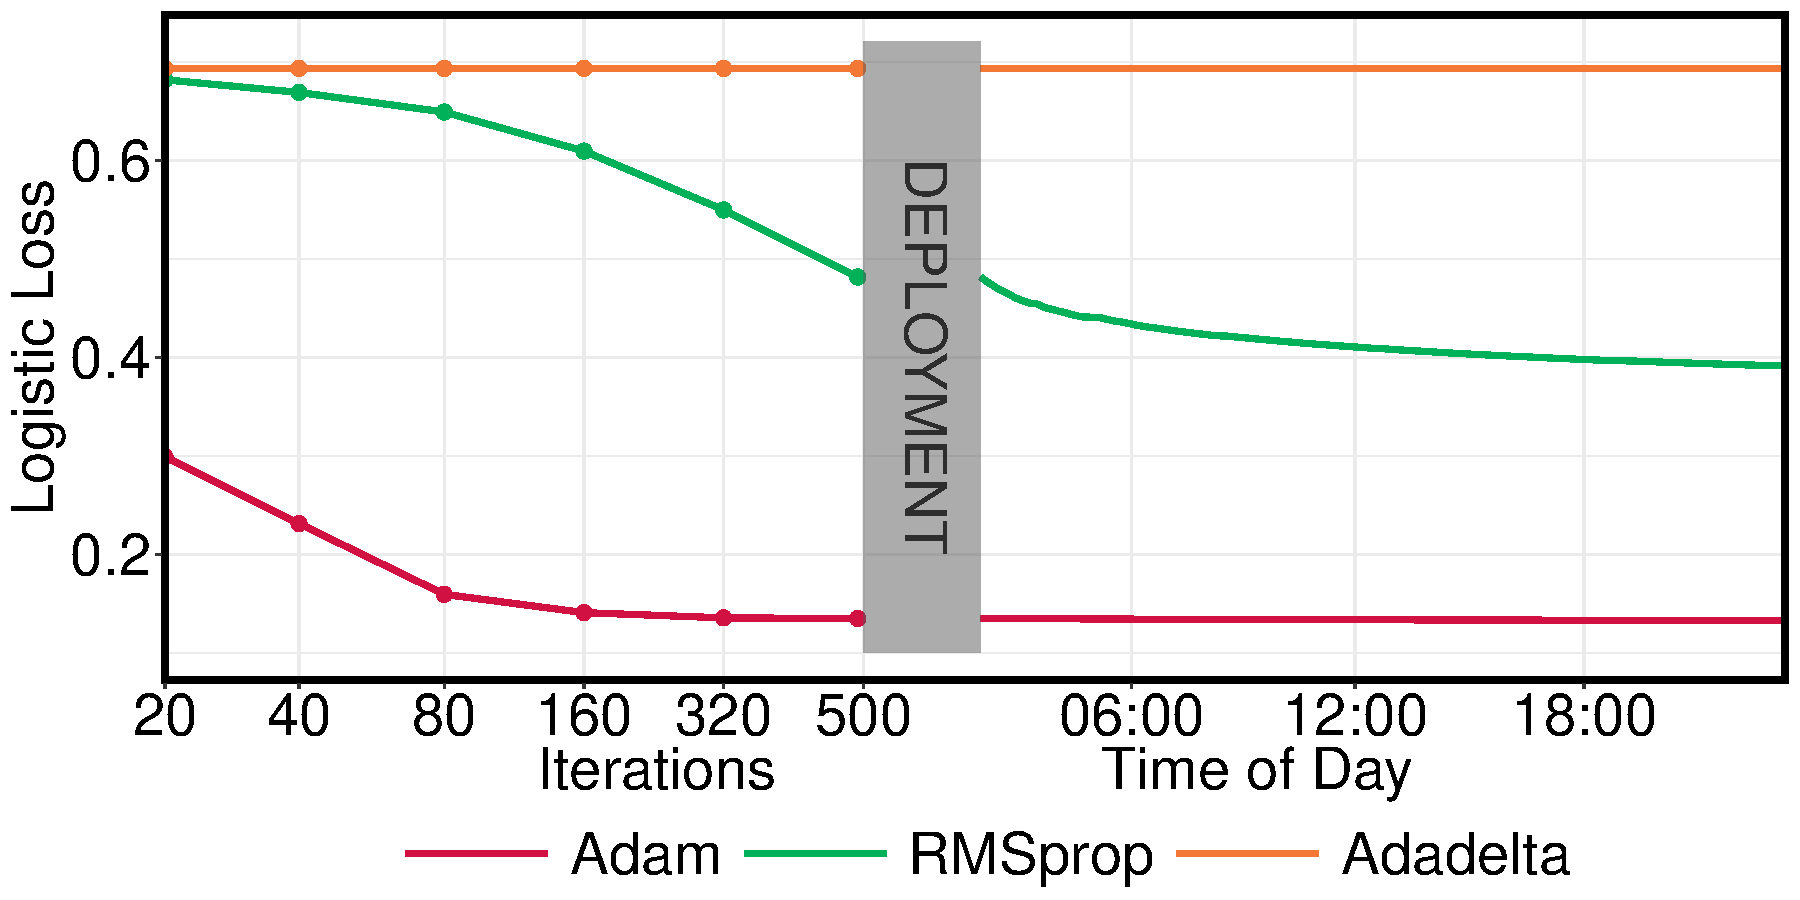
\includegraphics[width=\columnwidth]{../images/experiment-results/criteo-learning-rate-experiment.pdf}
\caption{Learning rate adaptation techniques for Criteo pipeline}
\label{fig:criteo-learning-rate}
\end{figure}

Adadelta performs very poorly during the offline training phase.
The Criteo dataset is a complex and high dimensional data, where features are a mix of numerical and categorical variables.
Since categorical features are not standardized, Adadelta is not able to effectively tune the learning rate for a mix of standardized and non-standardized features.
Similar to the offline SGD training, Adadelta performs poorly for proactive training after the model is deployed.
In fact, the error rate of the model, starting from the 20th iteration to end of day 1, stays almost constant throughout the experiment.

Unlike Adadelta, RMSprop reduces the error rate on the evaluation dataset through the offline SGD training.
Before the deployment, the error rate of the model is dropped to $0.48$.
Similarly, after the deployment, proactive training of the model using RMSprop reduces the error rate by $18\%$.

Adam has the best performance among the evaluated learning rate adaptation techniques.
Using Adam, the model fully converges after 500 iterations of SGD during the offline training phase.
After the deployment, the error rate is further reduces by $1.4\%$.
While the reduction in error rate for Adam is smaller than RMSprop, Adam still outperforms RMSprop after a day of proactive training of the model.

This experiment shows that choosing the process of choosing the learning rate adaption technique for proactive training is similar to the process of choosing it for the offline SGD training.
A learning rate adaptation technique that performs best during the offline training of the model also has the best performance for proactive training, when the model is deployed.

While Adam performs the best for Criteo pipeline, this does not indicate that Adam is the best learning rate adaptation technique for proactive training for every other pipeline and model.
For every pipeline and dataset, the users have to evaluate the performance of the different learning rate adaptation techniques during the offline training of the model.
The method that performs best during the offline training also has the best performance for the proactive training.

\subsection{Sampling Methods}
In this section, we evaluate the effect different sampling modes on the quality of the model.
We use a sampling rate of $0.1\%$ for all the experiments where sampling is performed.
This sampling rate is chosen to be equal to the sampling rate used during the initial offline SGD training of the model.

Figure \ref{fig:sampling-mode-quality} shows how different sampling modes, namely random sampling, time-based random sampling, and no sampling, affects the quality of the model in Criteo pipeline.
In both random sampling and time based random sampling modes, first the data is sampled and then the new training data that has arrived at the system recently is appended to this sample and used in the proactive training.
In no sampling mode, only the recently arrived data is used in the proactive training.
In random sampling approach, the entire historical data is used for creating the sample.
In this scenario, the logistic error rate decreases in a very slow manner over time.
Since the deployed model is already fully trained on the historical data, using the historical data in the continuous training of the model does not have a big impact on the model quality.

The time-based sampling has a larger impact on the quality of the model.
We evaluated the quality of the model for one day and half day time intervals.
Using an interval of one day decreases the error rate by around 0.03\% more than when using the simple random sampling (entire historical data).
Moreover, decreasing the interval length results in a model with lower logistic error rate.
In our experiment, using a time interval of half day for the time-based sampling results in an error rate that is 0.14\% smaller than when using the simple random sampling. 
Disabling sampling completely has the biggest impact on the error rate as it decreases it by 1.3\%.

This experiment shows that the sampling window size has a big impact on the quality of the deployed model.
For Criteo pipeline, the dataset has a stable distribution, which stays the same throughout the course of the experiment.
As a result, limiting the training to the more recent data exposes the model to newer and unseen data which results in bigger changes (toward convergence) in the weights of the model (e.g., no sampling).
When the distribution of the incoming training data is stable, using more historical data to continuously train the model has little effect as the combination of historical and new data dampen the effects of the new data on the model and as a result the improvement in the model convergence is very small (e.g., sampling from the entire history).

\begin{figure}[h!]
\centering
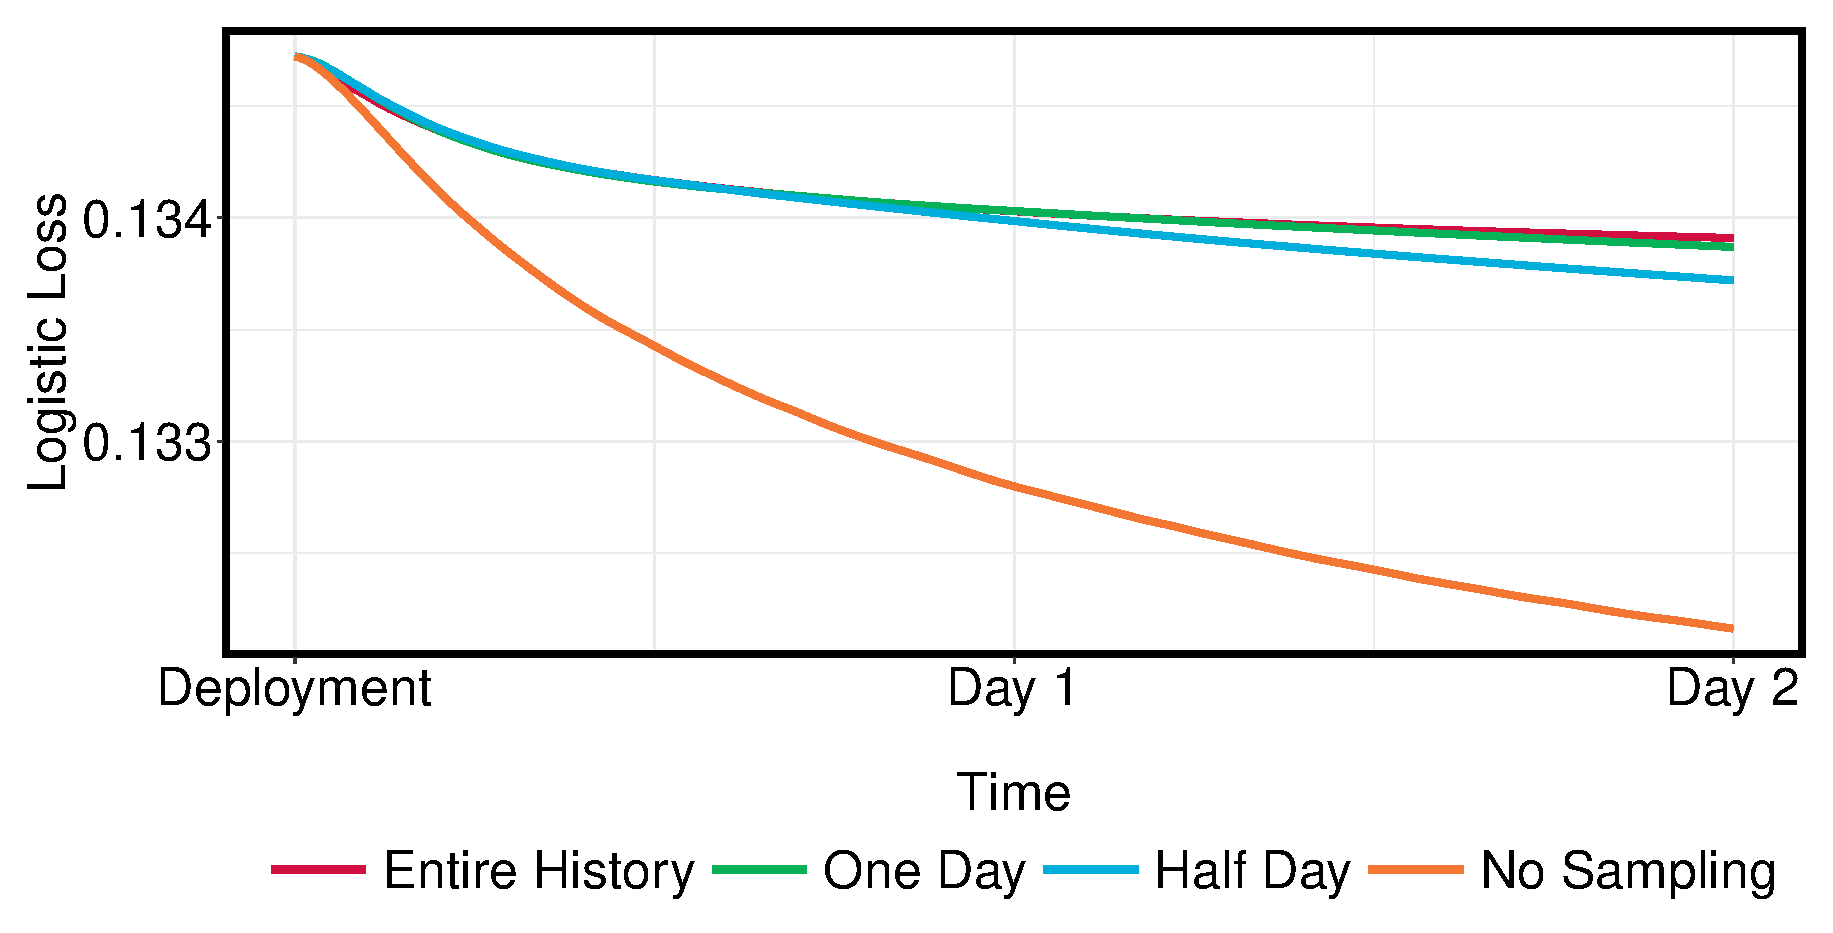
\includegraphics[width=\columnwidth]{../images/experiment-results/criteo-sampling-mode-experiments.eps}
\caption{Effect of different sampling modes on quality}
\label{fig:sampling-mode-quality}
\vspace{2mm}
\end{figure}

\begin{figure}[h]
\begin{subfigure}{\columnwidth/2}
\centering
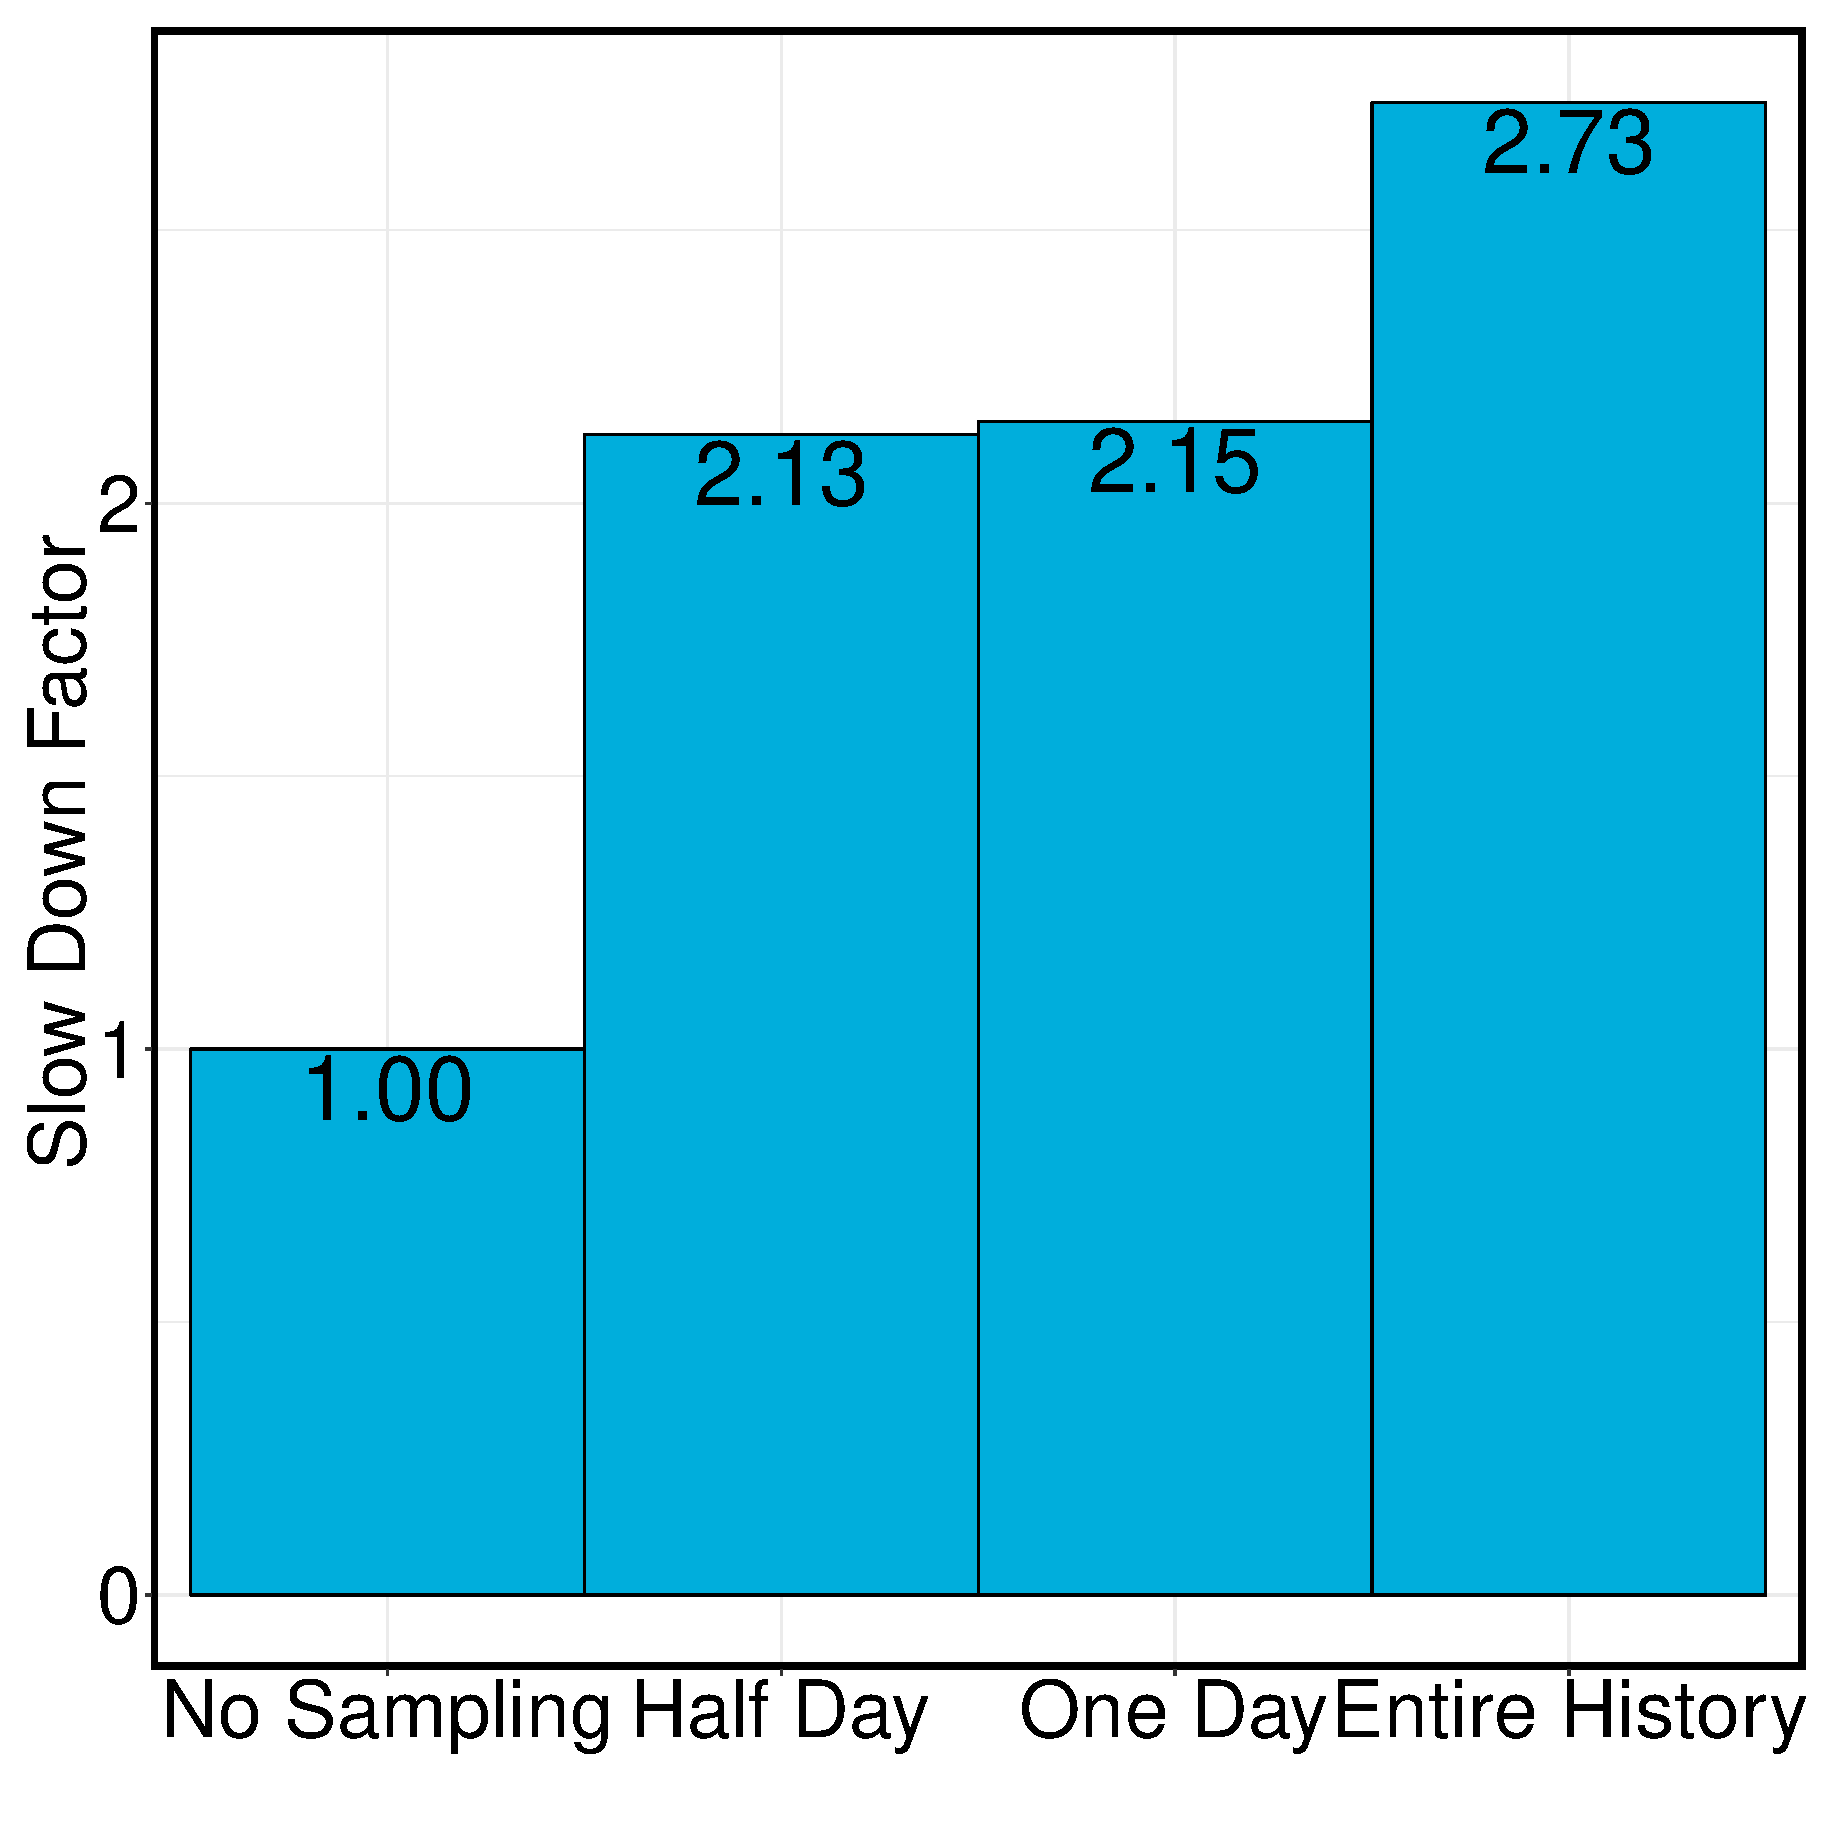
\includegraphics[width=\columnwidth]{../images/experiment-results/criteo-sampling-total-experiment.eps}
\caption{Total time}
\label{fig:sampling-mode-total-time}
\end{subfigure}%
\begin{subfigure}{\columnwidth/2}
\centering
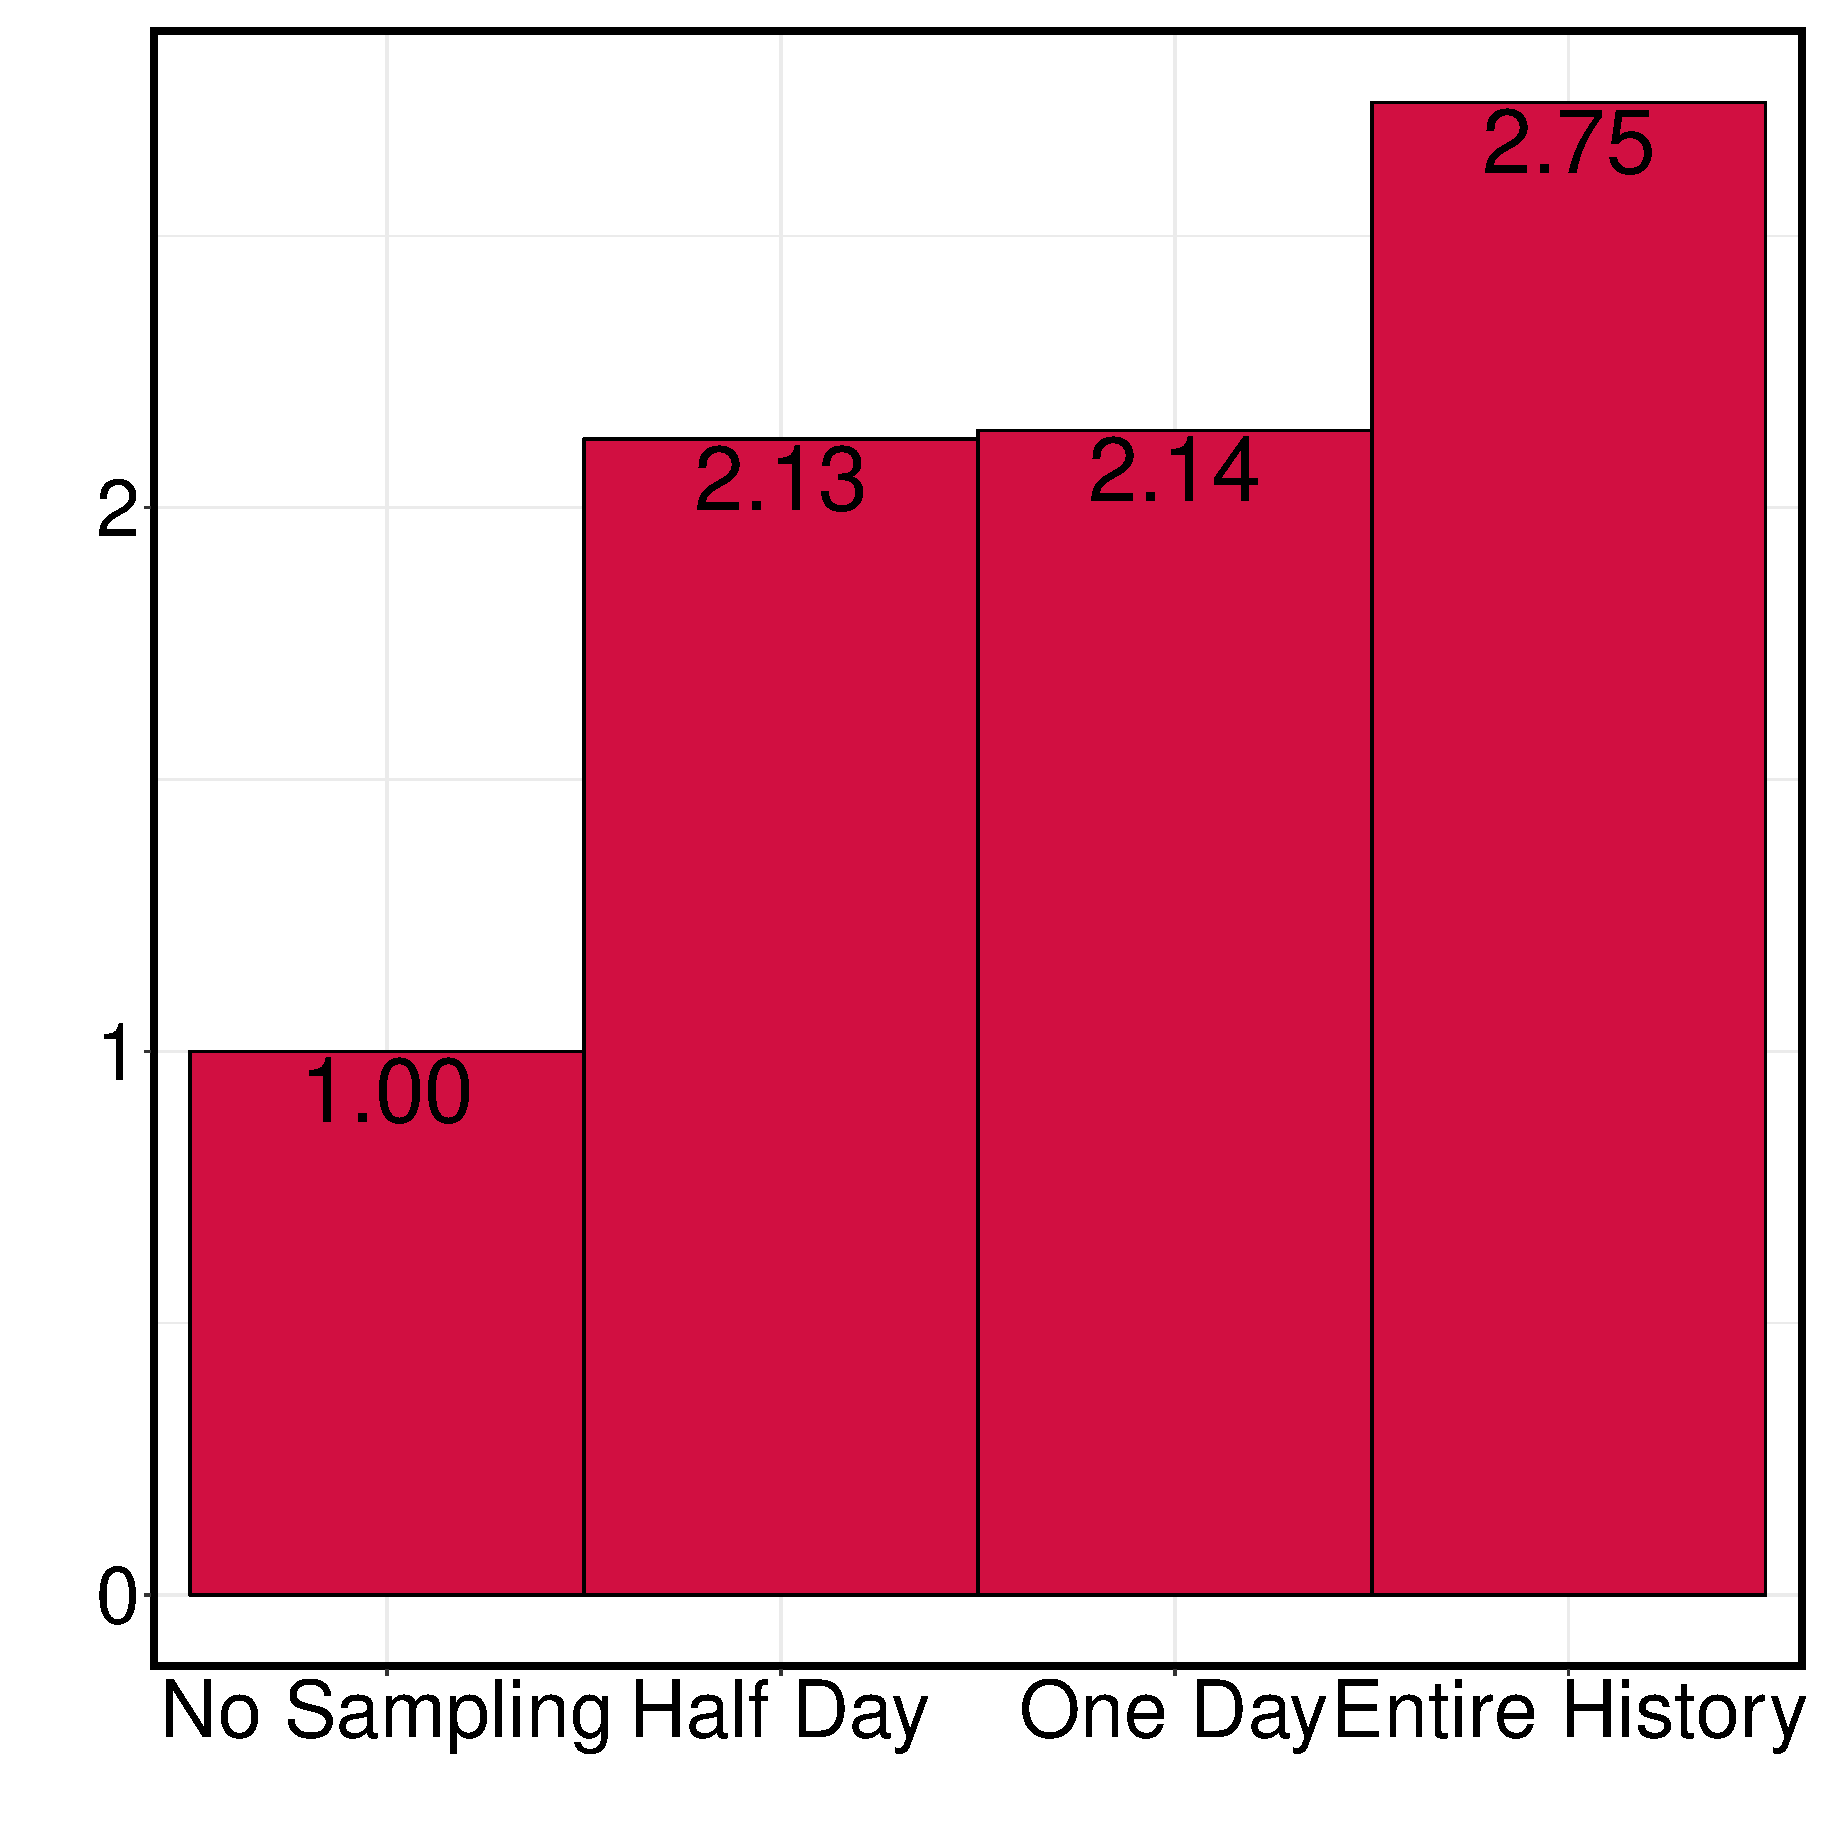
\includegraphics[width=\columnwidth]{../images/experiment-results/criteo-sampling-data-experiment.eps}
\caption{Data processing time}
\label{fig:sampling-mode-data-time}
\end{subfigure}
\vspace{2mm}
\caption{Slow down factor of different sampling approaches}
\label{fig:sampling-mode-time}
\end{figure}

Figure \ref{fig:sampling-mode-time} shows the effect of different sampling methods on the training time of the pipeline.
Figure \ref{fig:sampling-mode-total-time} shows that using time-based sampling (intervals of one and half a day) and simple random sampling (the entire history) increases the total training time by a factor of $2.13$ to $2.73$ over when no sampling is performed.
However, the slow down in training time is not due to the sampling operations.
To demonstrate this, for each sampling method, we also capture the amount of time the deployment platform spends in processing the data after the sample is provided by the data manager.
The slow down factor for both data processing and the total time is almost identical.
This demonstrates that our data manager is able to provide the samples (either from a limited time interval or the entire history) very efficiently without inuring additional overhead.

The data manager partitions the incoming data and stores the partitions using a time stamp.
When a sample is required, the data manager directly samples the partitions instead of the actual data point.
This technique allows us to perform time-based and simple random sampling without requiring a scan of the data.

\subsection{Scheduling Policy}
In this section, we analyze the scheduling policy of our deployment platform.
In our prototype, we simulated 2 days of continuous training of Criteo data using Apache Spark.
Since the streaming component of Apache Spark requires a fixed interval for executing mini batches, we set out to analyze the effect of our scheduling policy empirically.

Figure \ref{fig:scheduling-policy-time} shows the actual execution time of every proactive training instance throughout the simulation.
The execution time of proactive training ranges from $23$ seconds to $53$.
In our estimation, we use a \textit{slack} parameter of $10$.
We estimate the throughput and latency based on the time it takes for the deployment platform predict the labels of the evaluation dataset.
The evaluation dataset contains around 2 million data points.
The deployment platform is queried using the evaluation dataset every minute and requires $15$ seconds to return the predictions (when the evaluation dataset is stored on disk). 
This amounts to a latency of $7 * 10 ^ {(-6)}$ seconds (7.5 micro seconds) and throughput of $34,000$ requests per second.
Figure \ref{fig:scheduling-policy-time}  shows the scheduling intervals for every execution of the proactive training.

\begin{figure}[h!]
\centering
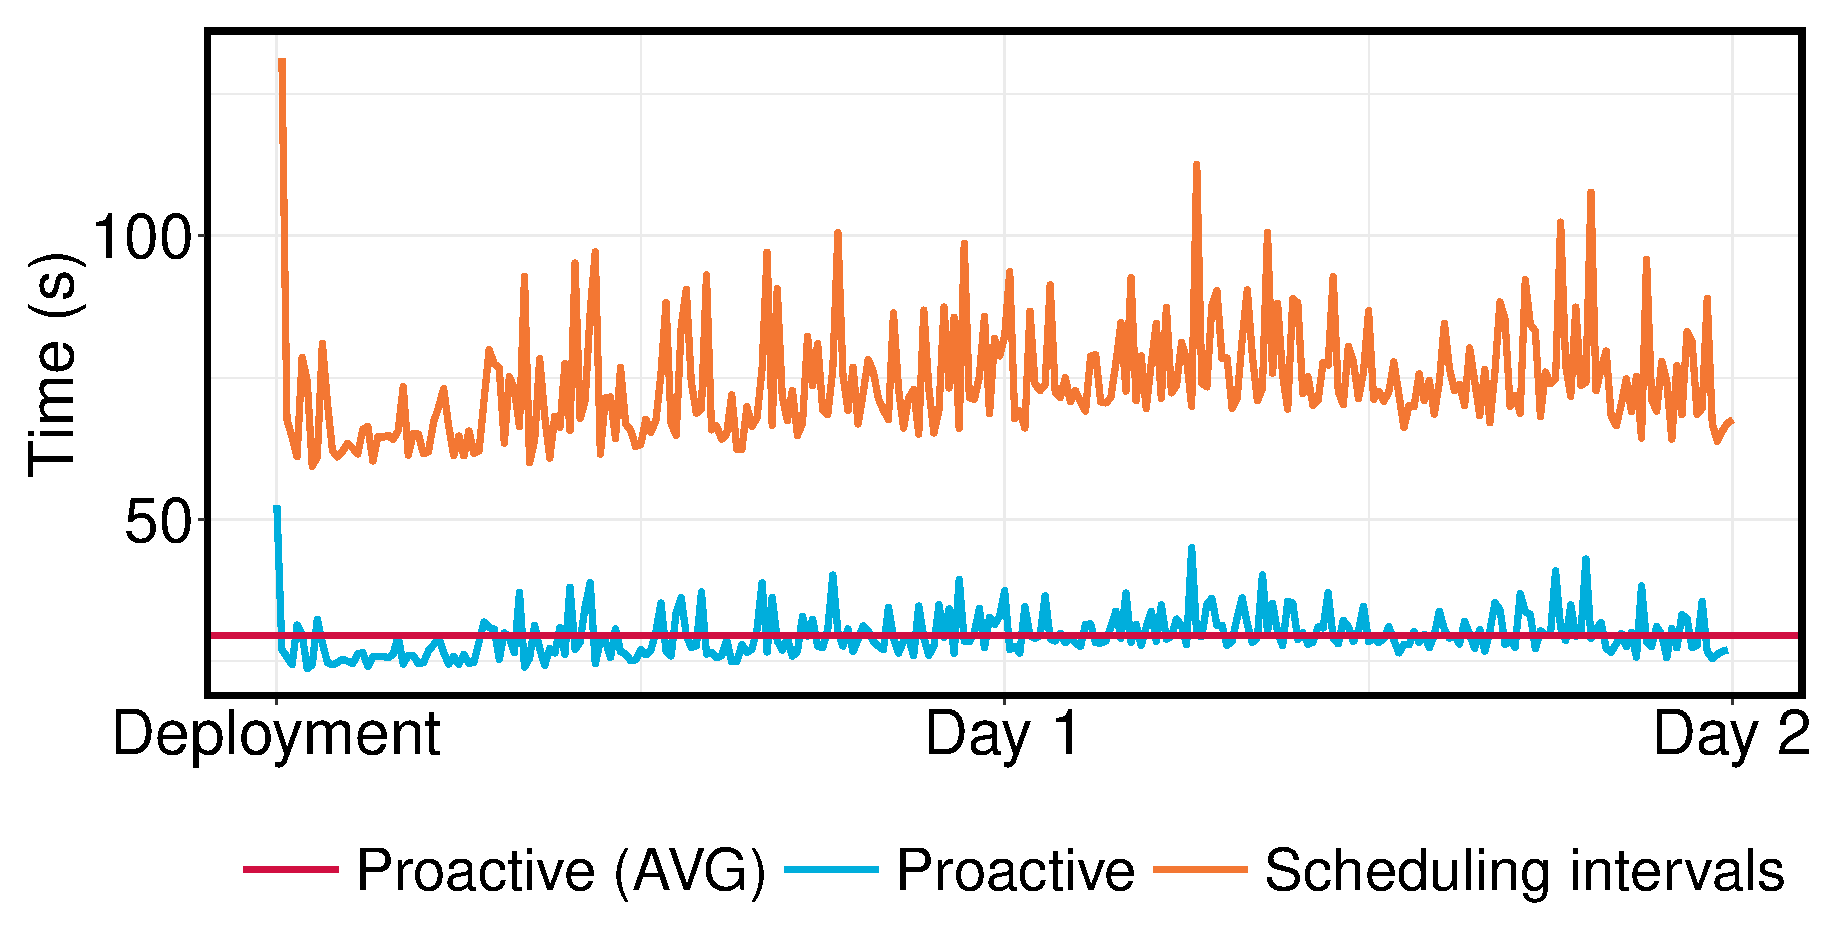
\includegraphics[width=\columnwidth]{../images/experiment-results/criteo-scheduling-experiment.eps}
\caption{Analysis of scheduling policy}
\label{fig:scheduling-policy-time}
\vspace{2mm}
\end{figure}

Our scheduler uses a very conservative formula to compute the scheduling intervals for instances of proactive training.
Using the slack parameter, we can guide the scheduler to increase or decrease the scheduling interval until the next proactive training.
The slack parameter allows for the deployment platform to accommodate surges in the incoming prediction requests and new training data.
In scenarios that sudden surges are expected (e.g., online stores), we recommend a large slack parameter (recommended value is $10$). 


\subsection{Model Freshness}\label{subsec:model-freshness}
We measure model freshness by two metrics: training recency and rate of new features.
Training recency is determined by the scheduling rate.
Performing more frequent training results in models that can adapt to changes in the data more rapidly.
In Criteo pipeline, we use a feature encoder to transform the categorical features into binary indicator variables.
The initial training data (Day 0) only contains a small portion of all the unique categorical features of the Criteo dataset.
The incoming training data may contain features that have not existed in the dataset before.
Figure \ref{fig:criteo-feature-discovery} shows the feature size over time for the first 5 days after deployment of Criteo pipeline.
The rate of incoming new features is roughly 30,000 per minute and every day around 45 million new features are generated.

Using our continuous training approach, we update the pipeline as soon as new features become available.
During the next scheduled proactive training, the model is updated using these new features.
As a result, the deployed pipeline is able to answer prediction queries that may contain the same set of features more accurately.
Using a daily training approach, any unseen features that arrive at the system are dropped before a prediction is made.

\begin{figure}[H]
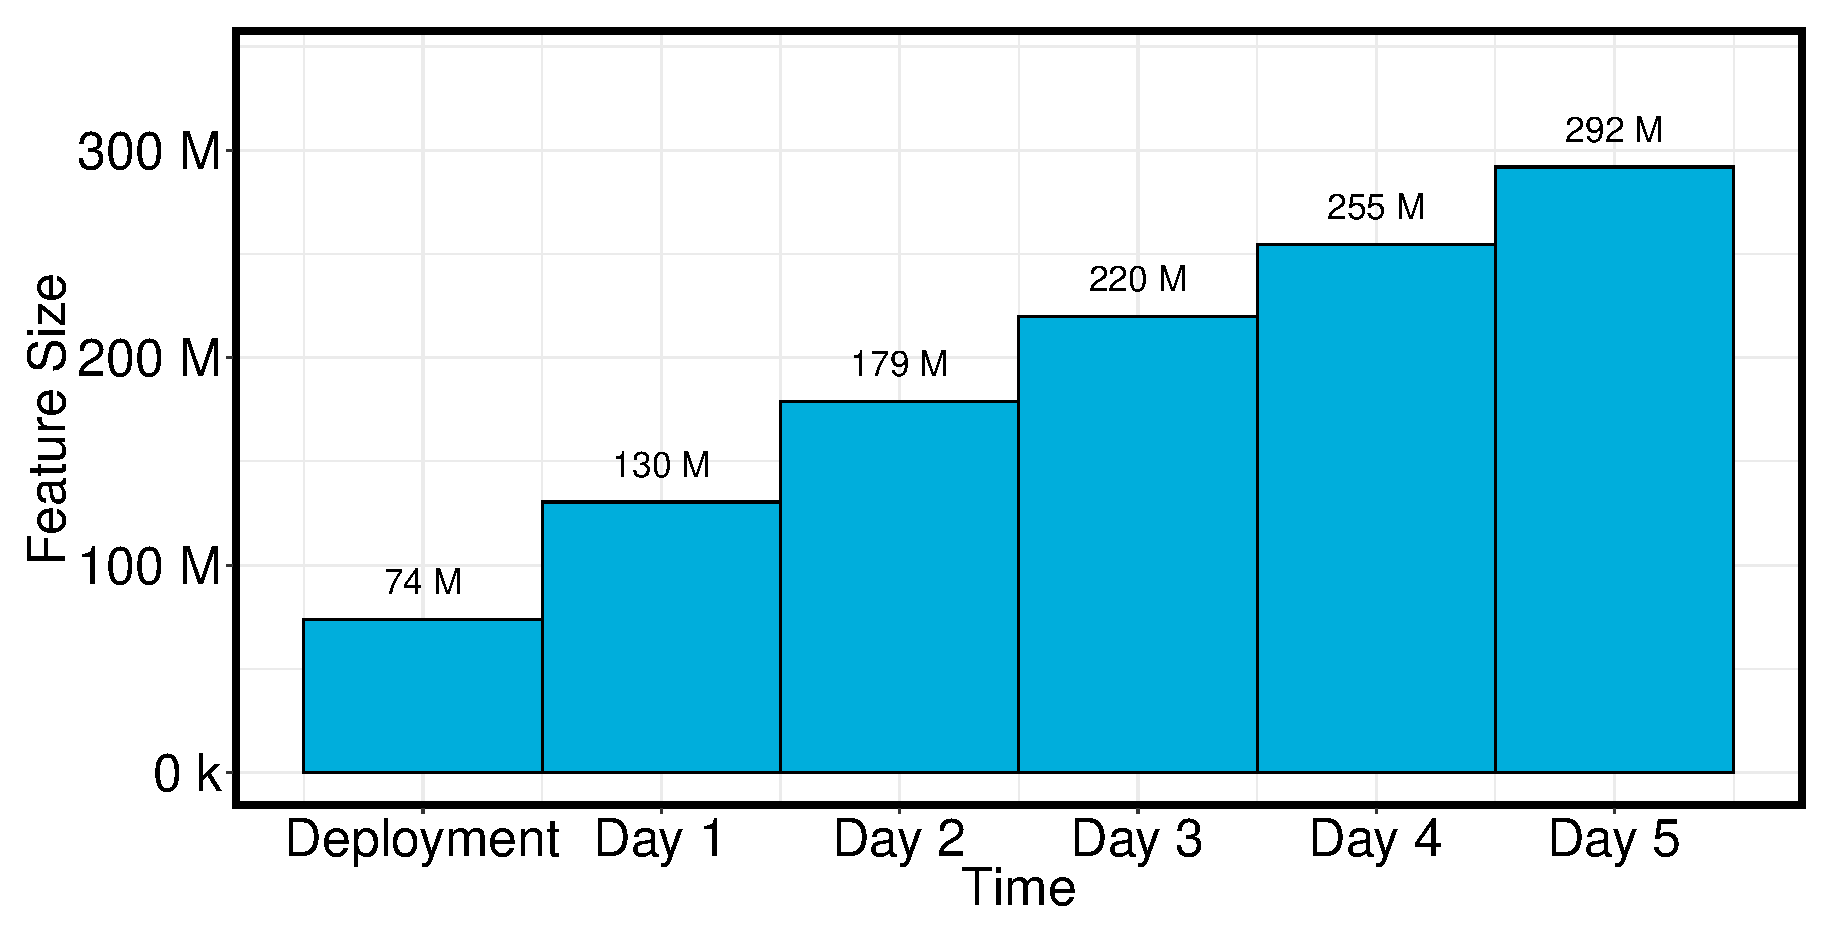
\includegraphics[width=\columnwidth]{../images/experiment-results/criteo-feature-discovery-experiment.eps}
\caption{Criteo categorical feature size over time}
\label{fig:criteo-feature-discovery}
\end{figure}


\subsection{Proactive Training}
In this section, we evaluate the quality of the deployed model.
Figure \ref{fig:loss-proactive-vs-daily} shows the logistic loss of the continuous training and periodical approaches on the Criteo pipeline.

After the deployment, the continuous training updates the pipeline and train the model using the incoming training iterations.
The incoming data contains both unseen training observations and new features, as described in experiment \ref{subsec:model-freshness}.
The continuous training approach trains the model over this data within a short period of time which results in a high quality and fresh model.

To measure the performance of periodical training approach, we train the model at the end of every day of the simulation.
The initial training and periodical training use the same set of parameters required by SGD.
We use Adam learning rate adaptation technique and sampling rate of $0.1$ for training the initial and periodical training of the pipeline.

The initial deployed model converges after 500 iterations.
However, after day 1, the amount of data stored data is doubled, and training the model $500$ iterations results in a model that has an error rate of $0.002$ higher than the initial model.
Because of the larger number of data points, the periodical training has to train the model longer in order to achieve a lower error rate.
To decrease the error rate of the model further, we train the model for $2000$ iterations.
However, continuous training still outperforms periodical training.
The error rate of the model trained using continuous training is $1.6\%$, $0.9\%$, and $0.15\% $ lower than a model trained using periodical training using $500$, $1000$, and $2000$ iterations respectively at the end of the day 1 of the simulation.

We observe a similar behavior for the second periodical training.
Because of the large training dataset after the second day of the simulation, the model requires a longer training period to converge.
After two days of training, the continuous training approach results in an error rate that is smaller than the error rates of a model trained using 500, 1000, and 2000 iterations by $3.4\%$, $2.8\%$, and $2.2\%$.

This experiment shows that the continuous training of a machine learning pipeline decreases the error rate while still producing fresher models when compared to the periodical training of the pipeline.
It has to be noted that the poor performance of periodical training after each day can be alleviated by more advanced training methods or better parameter selection for the underlying SGD optimization algorithm.
In this experiment, we demonstrate that using the same set of parameters (learning rate and sample size), we are able to achieve a lower error rate by using continuous training approach.
In a real deployment scenario, when the quality of the model degrades after the periodical training, either the model is discarded or it is trained for a longer period of time using more sophisticated training algorithm, while the existing model continuous to answer prediction requests.


\begin{figure}[h!]
\centering
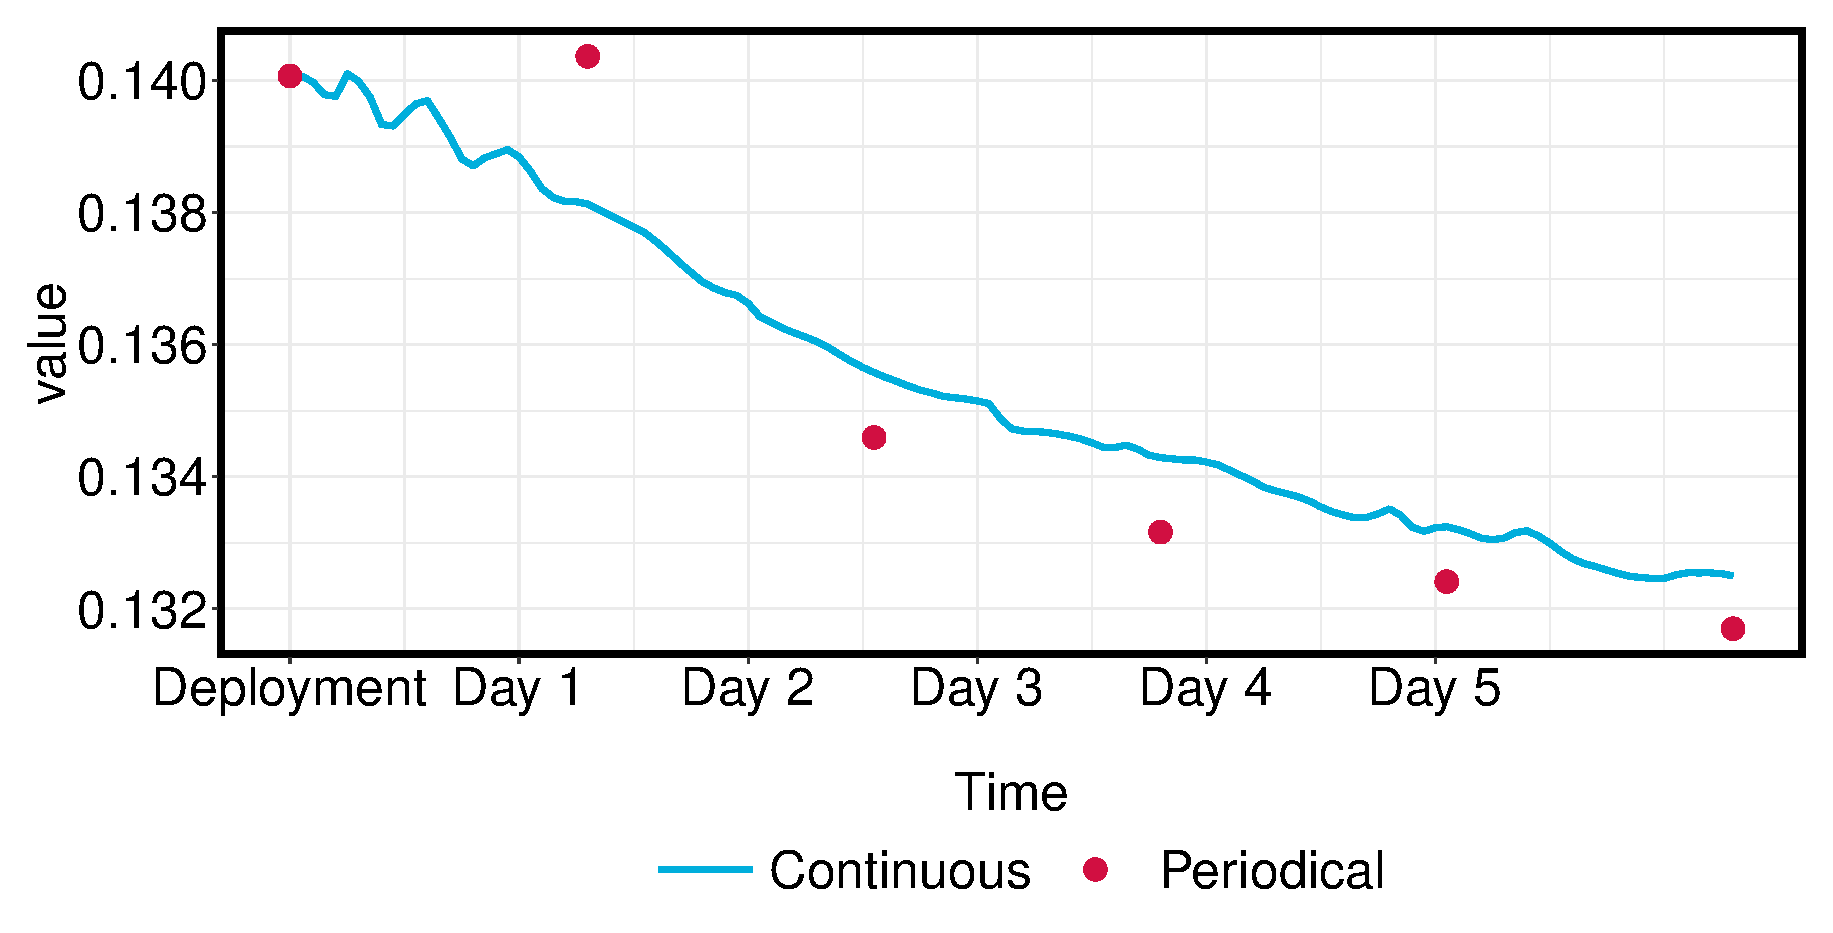
\includegraphics[width=\columnwidth]{../images/experiment-results/criteo-proactive-training-experiment.eps}
\caption{Model quality for different deployment approaches}
\label{fig:loss-proactive-vs-daily}
\vspace{2mm}
\end{figure}

\subsection{Total Training Time}
In this section, the total training time for continuous and periodical deployment approaches are measured.
The total training time includes the time spent in pre-processing the training data using the pipeline components and training the model.
Similar to previous experiments, for periodical training, we train the model for 500 iterations at the end of each period.

Figure \ref{fig:training-time-deployment} shows the total training time of the Criteo pipeline for different deployment approaches.
Using continuous training, the time spent in training is smaller than that of periodical training by a factor of $5$.
This is due to the large of amount of redundant data processing and model training that exists in periodical training approach.
In the periodical training, the underlying pipeline is trained from scratch every day, which includes ingesting the data, performing the data transformation steps of the pipeline and finally training the model using the transformed data.
However, in continuous training, the pipeline is incrementally updated when new data arrives at the system.
Moreover, the total training time can be further reduced in the continuous training approach by switching on the online statistics update and materialization optimizations.
Figure \ref{fig:training-time-optimization} shows the effect each optimizations on the continuous training approach.
By enabling online statistics update, the pipeline components are updated when new training data becomes available.
Therefore, the proactive trainer does not need to update pipeline components and proceeds to transform the data directly.
Enabling the online statistics update optimization reduces the total training time by a factor of $3$.
Moreover, enabling both online statistics and materialization allows the proactive trainer to skip the data processing part of the pipeline completely and directly proceeds to the model training, which only accounts for a small fraction of the pipeline.
Our experiment shows that enabling both online statistics update and materialization reduces the total training time by a factor of $18$, from $142$ to $8$ minutes.

\begin{figure}[h]
\begin{subfigure}{\columnwidth/2}
\centering
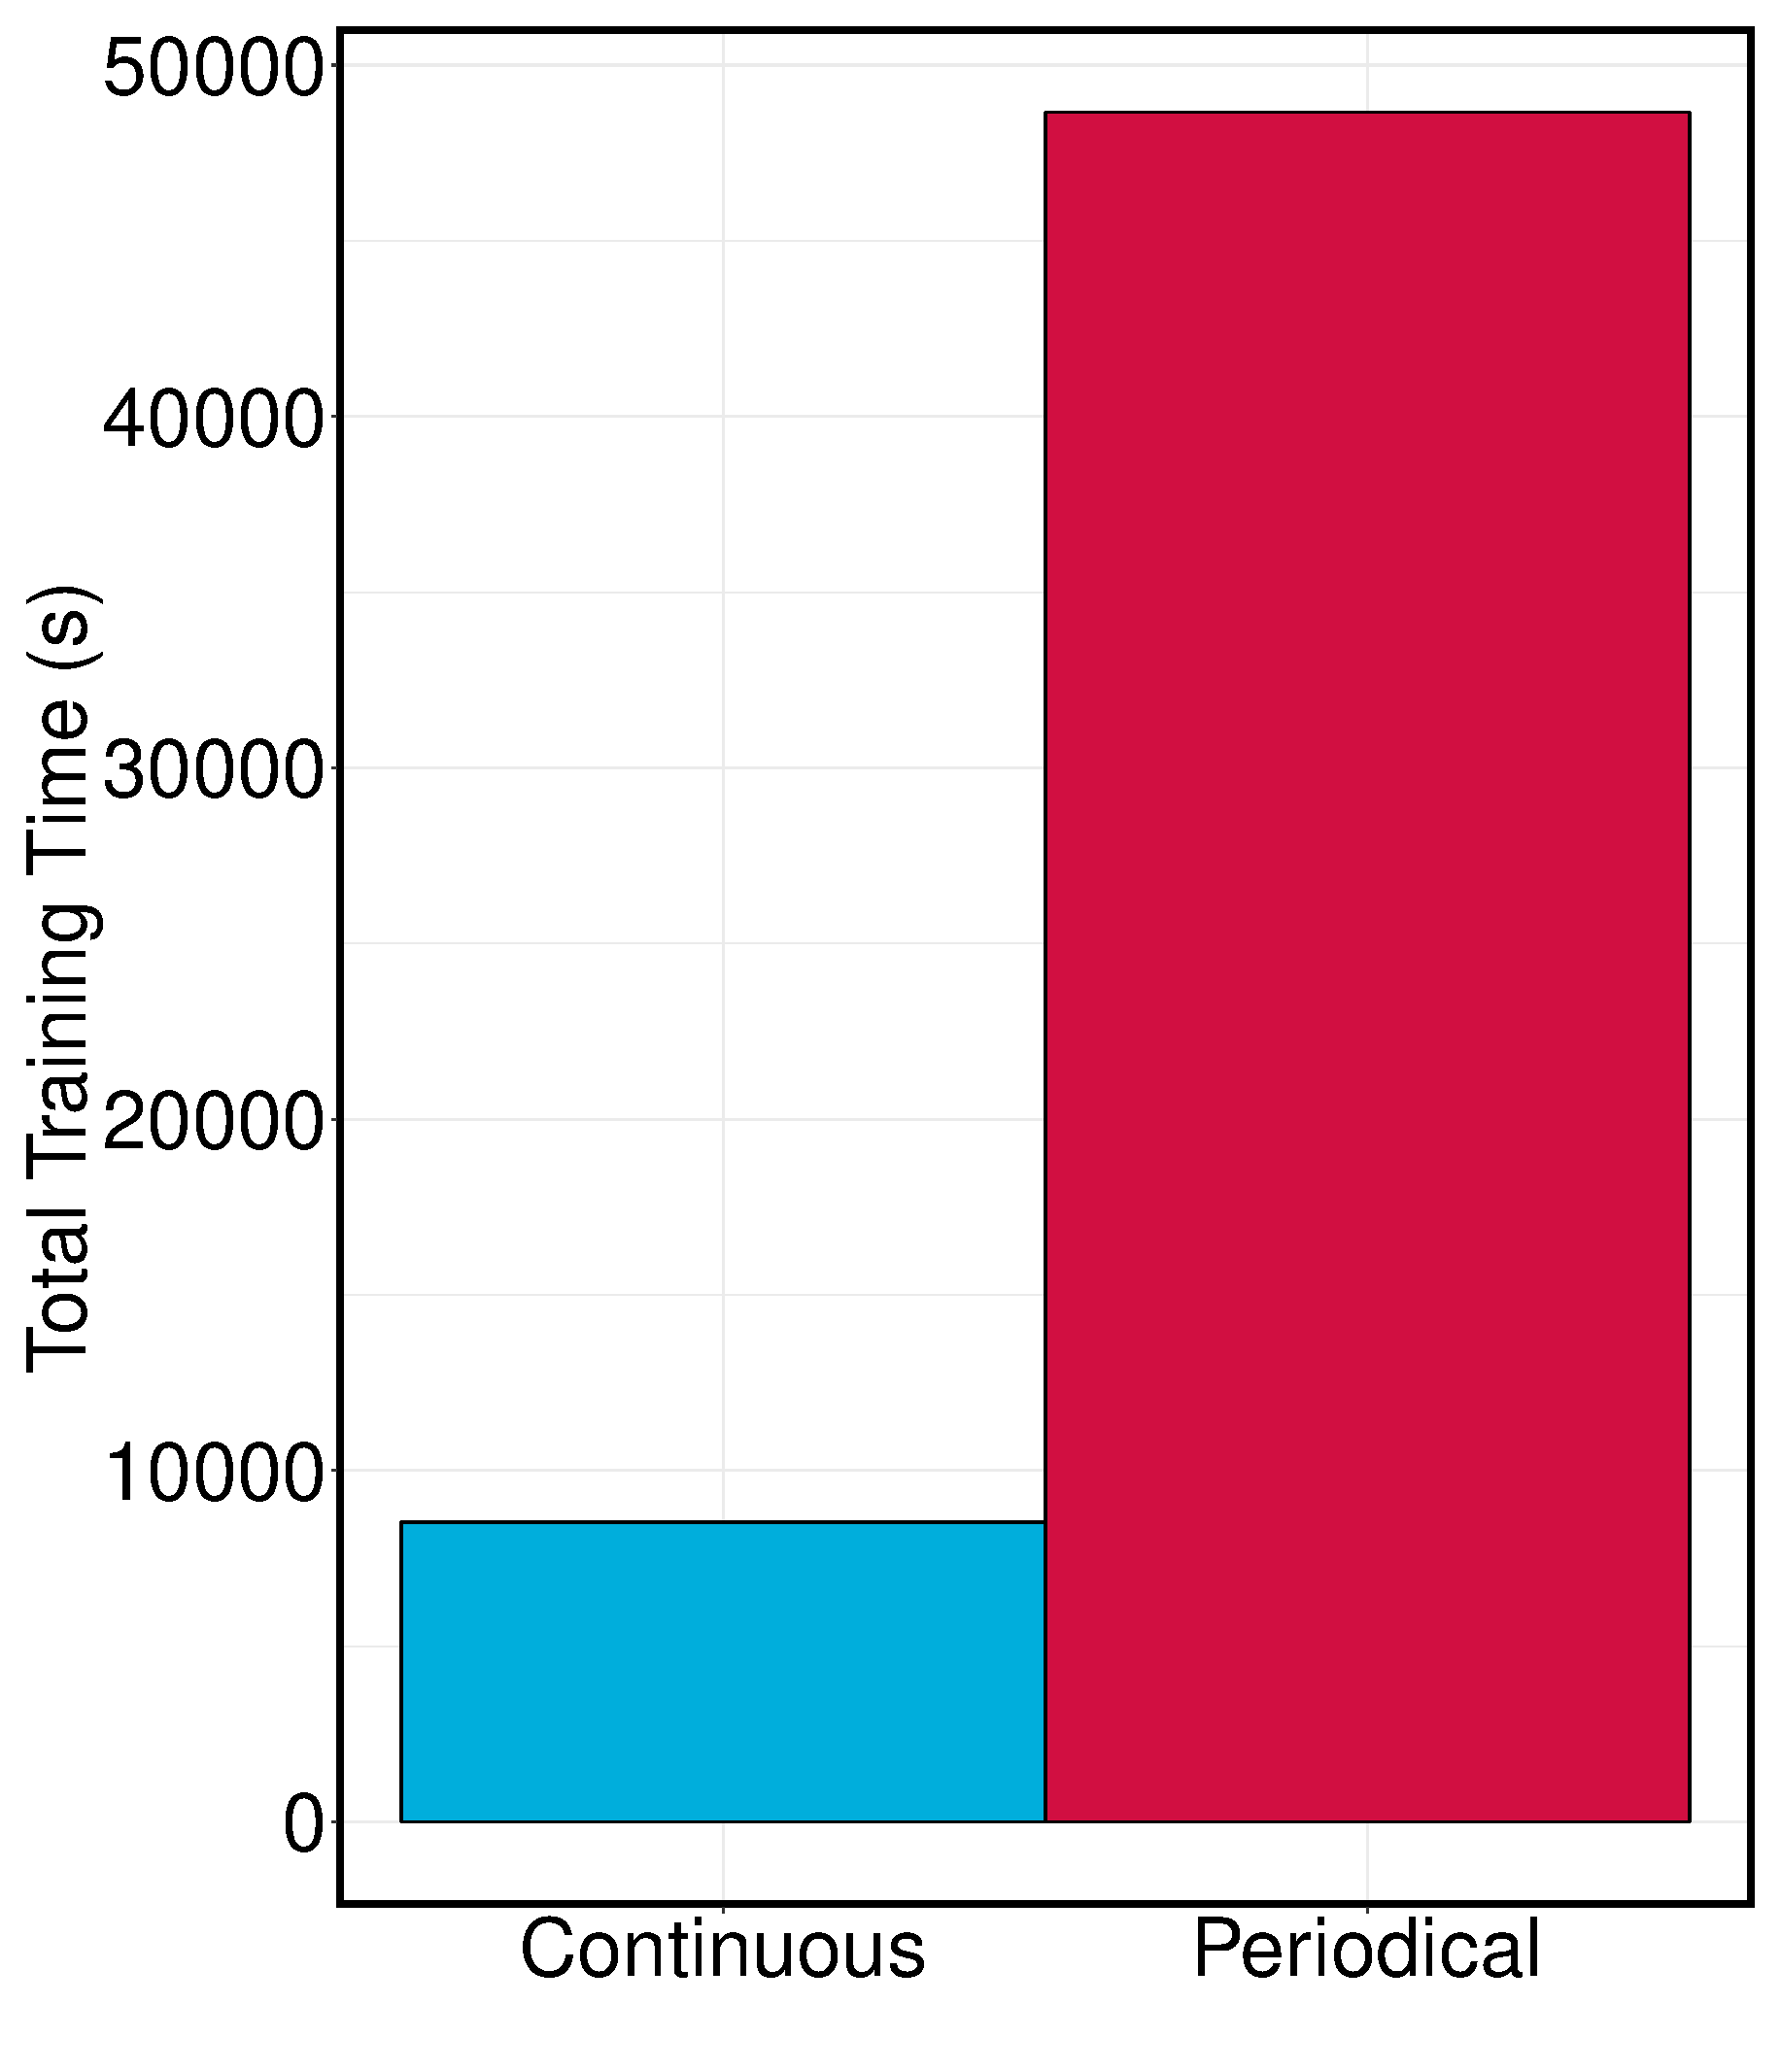
\includegraphics[width=\columnwidth]{../images/experiment-results/criteo-training-time-deployment-types-experiment.eps}
\caption{Deployment Approaches}
\label{fig:training-time-deployment}
\end{subfigure}%
\begin{subfigure}{\columnwidth/2}
\centering
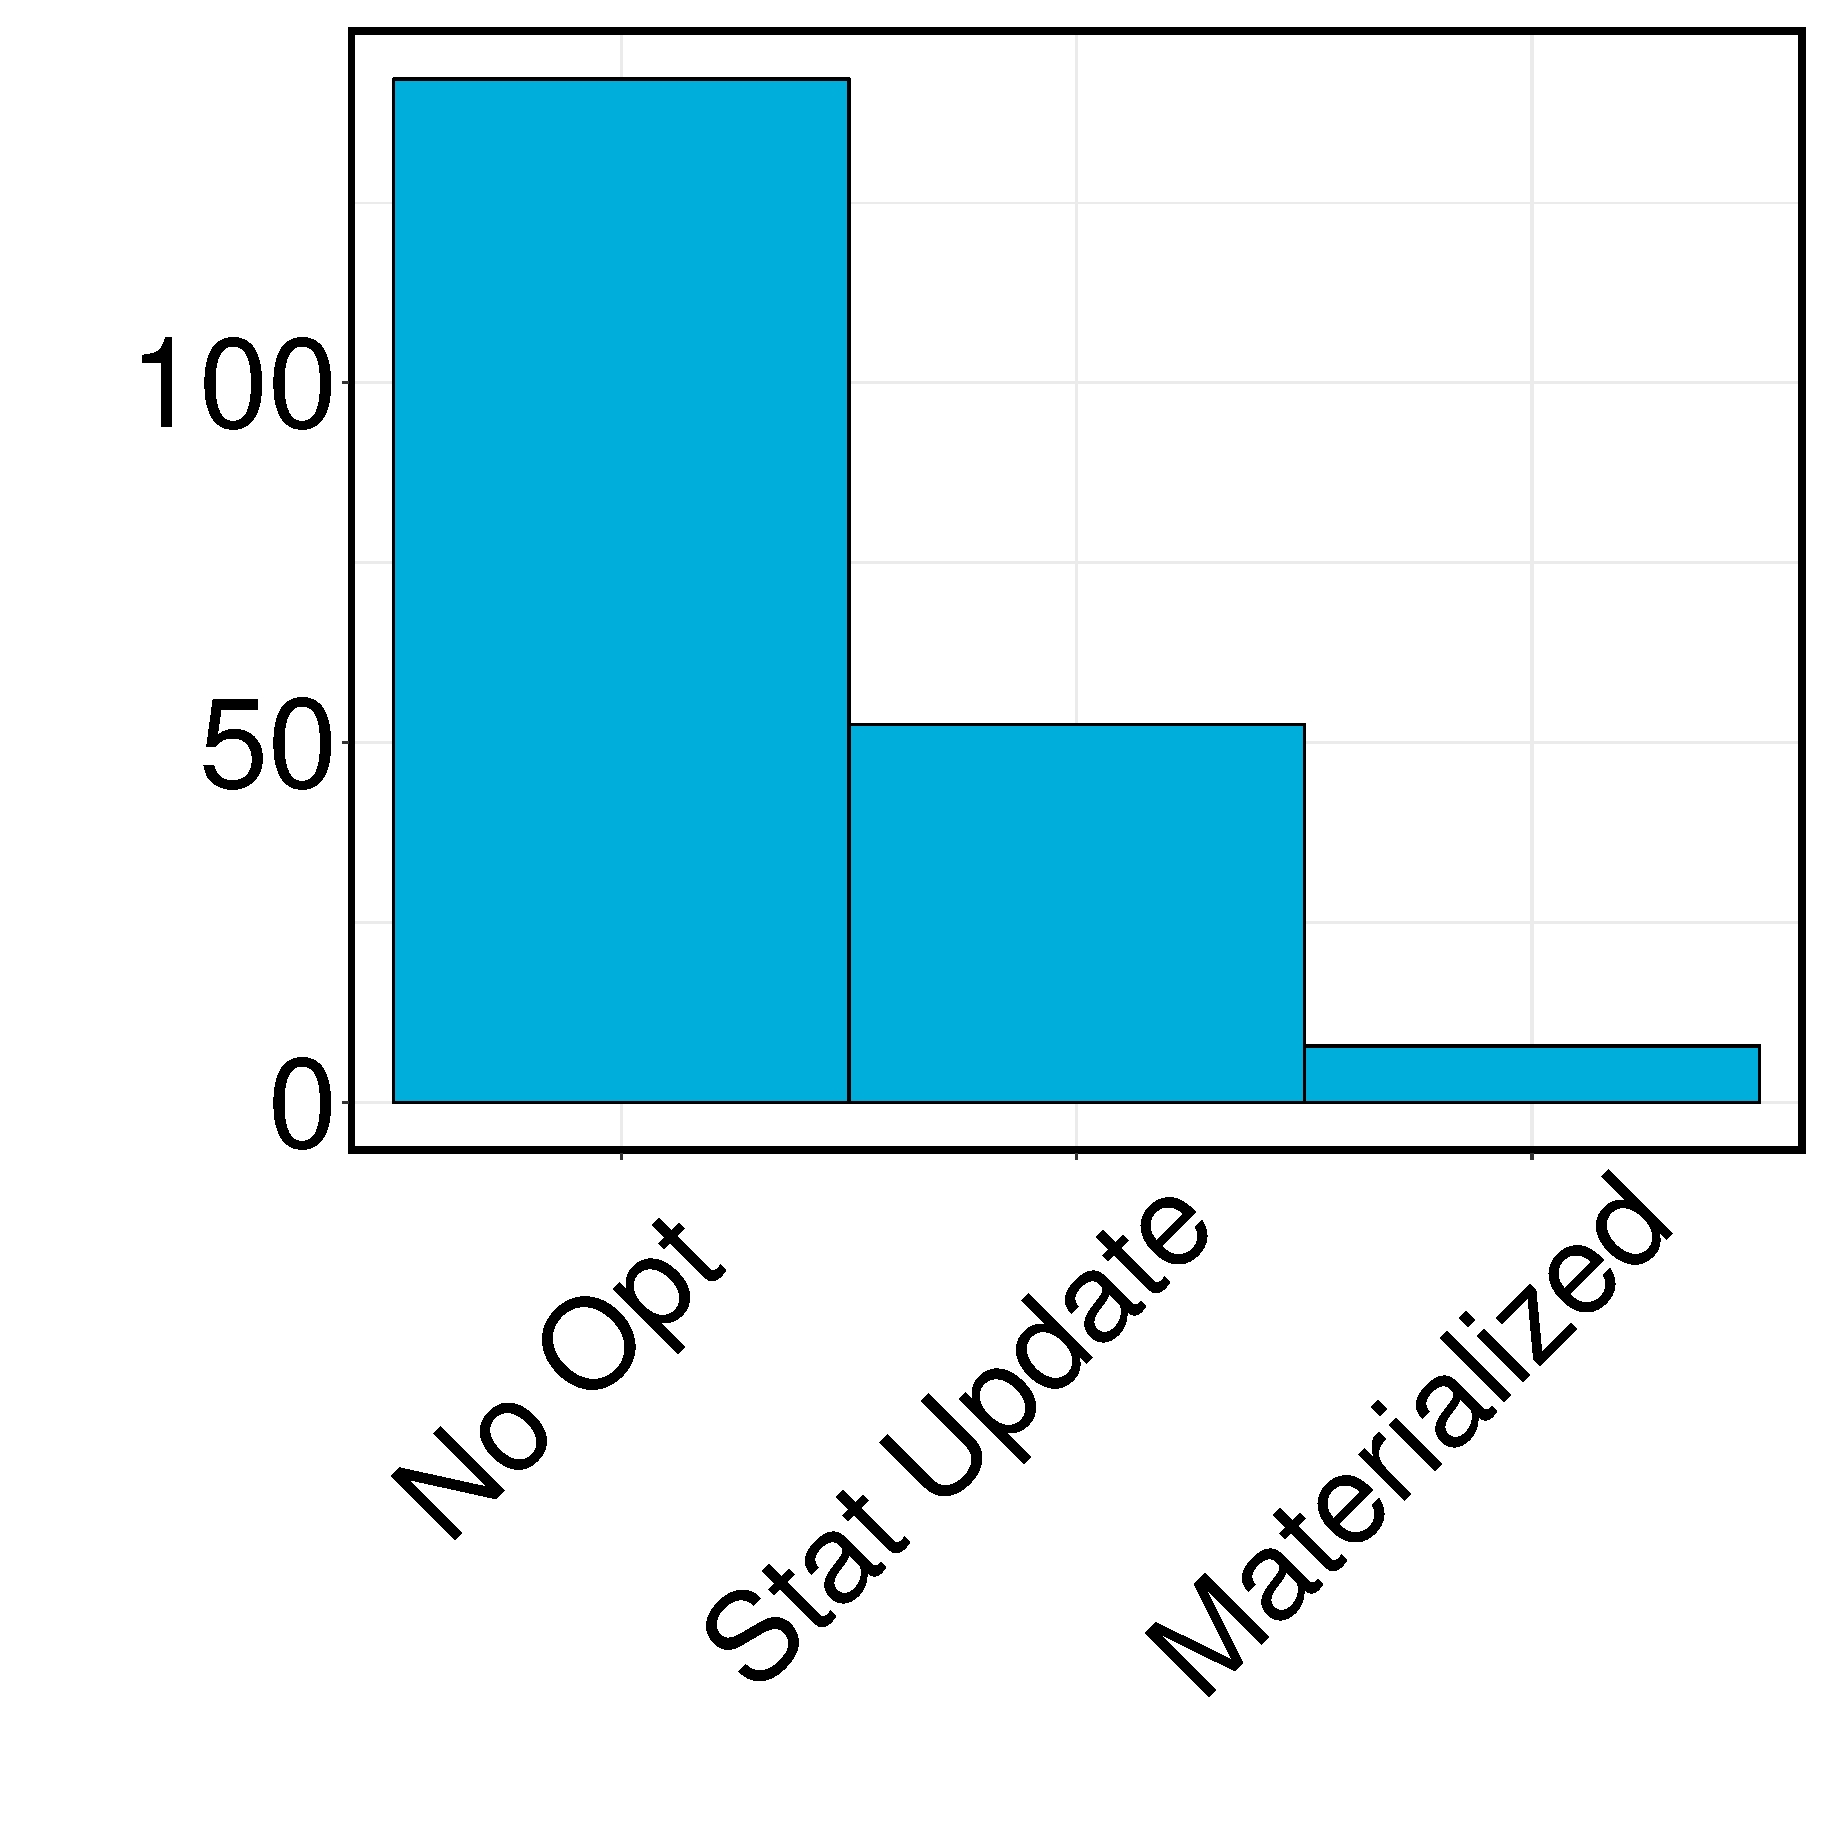
\includegraphics[width=\columnwidth]{../images/experiment-results/criteo-training-time-optimizations-experiment.eps}
\caption{Optimizations}
\label{fig:training-time-optimization}
\end{subfigure}
\vspace{2mm}
\caption{Total training time for different deployment approaches (with optimizations enabled)}
\end{figure}

One possible problem with the materialization optimization is the amount of space required to store the materialized dataset.
Depending on the type of the data processing the size of the materialized data may increase.
In our experiments, the input data is a combination of Integer and String values, however, after the pre-processing steps of the Criteo pipeline, the data is transformed to large vectors of Double.
As a result, the size of the materialized data increases by a factor of 2.

\subsection{Discussion} \label{subsec:discussion}
Our experiments show that continuous training approach outperforms periodical training of deployed models and pipelines.
By using proactive training we manage to reduce the average error rate by $1.6\%$.
As the amount of existing data increases after each time interval, periodical training requires more training iterations and more advanced techniques to train a model with an acceptable error rate.
Continuous training does not face the same issue as the periodical training since the existence of more training data does not require a change in the parameters of SGD or more frequent scheduled instances of proactive training. 

Our continuous training approach reduces the total training time by a factor of $5$ after two days of training.
Moreover, our online statistics computation and data materialization optimizations reduce the total training time by 2 orders of magnitude over the state of the art deployment approaches.
As the deployment process continuous, the training time for the continuous training approach increases linearly as the frequency of proactive training remains the same.
However, periodical training has to process larger datasets at the end of each time interval.

The frequent updates that the continuous training approach applies to the deployed model is the main reason for the reduction in error rate.
These frequent updates enable the model to adapt to the recently unseen data faster.
Moreover, the continuous training approach allows the model to be updated with new features, that were not present in the data before, faster than periodical training.
In periodical training, new features are only discovered after each training interval (e.g., 1 day for Criteo pipeline).
As a result, the deployment system discards the newly available features when answering prediction requests until the next training.

Proactive training is an extension of SGD optimization algorithm, where during each scheduled training an optional sample of the historical data and the newly available training data are combined and used to train the deployed model in-place.
Therefore, tuning proactive training is similar to the process of tuning SGD.
In our experiments, we show that the learning rate adaptation technique that works best with SGD during the offline training also results in the lowest error rate when used in the proactive training.

We show that our scheduling policy can effectively execute the proactive training and dynamically adapt to changes in the rate of incoming data, prediction latency, proactive training time, and sudden data surges.
We also demonstrate that how different sampling modes (simple random sampling, time-based sampling, and no sampling) affect the quality of the model.
Moreover, we use a data partitioning techniques to increase the efficiency of sampling operations.
Our experiments show that the using the data partitioning technique can effectively provide samples from different time intervals while incurring a small overhead.




